\chapter{Background}
 
\section{Coreference Resolution}
Coreference resolution is the task typically framed as identifying all mentions of entities and events in text and clustering them into equivalence classes \inlinecite{pradhan2012conll}. It is a task of identifying clusters of mentions referring to the same real-world entity. Furthermore, our machines even need to understand the coreference between sentences. It is an important step for a lot of higher level NLP tasks that involve natural language understanding such as document summarization, question answering, and information extraction.

\begin{figure}[H]
	\centering
	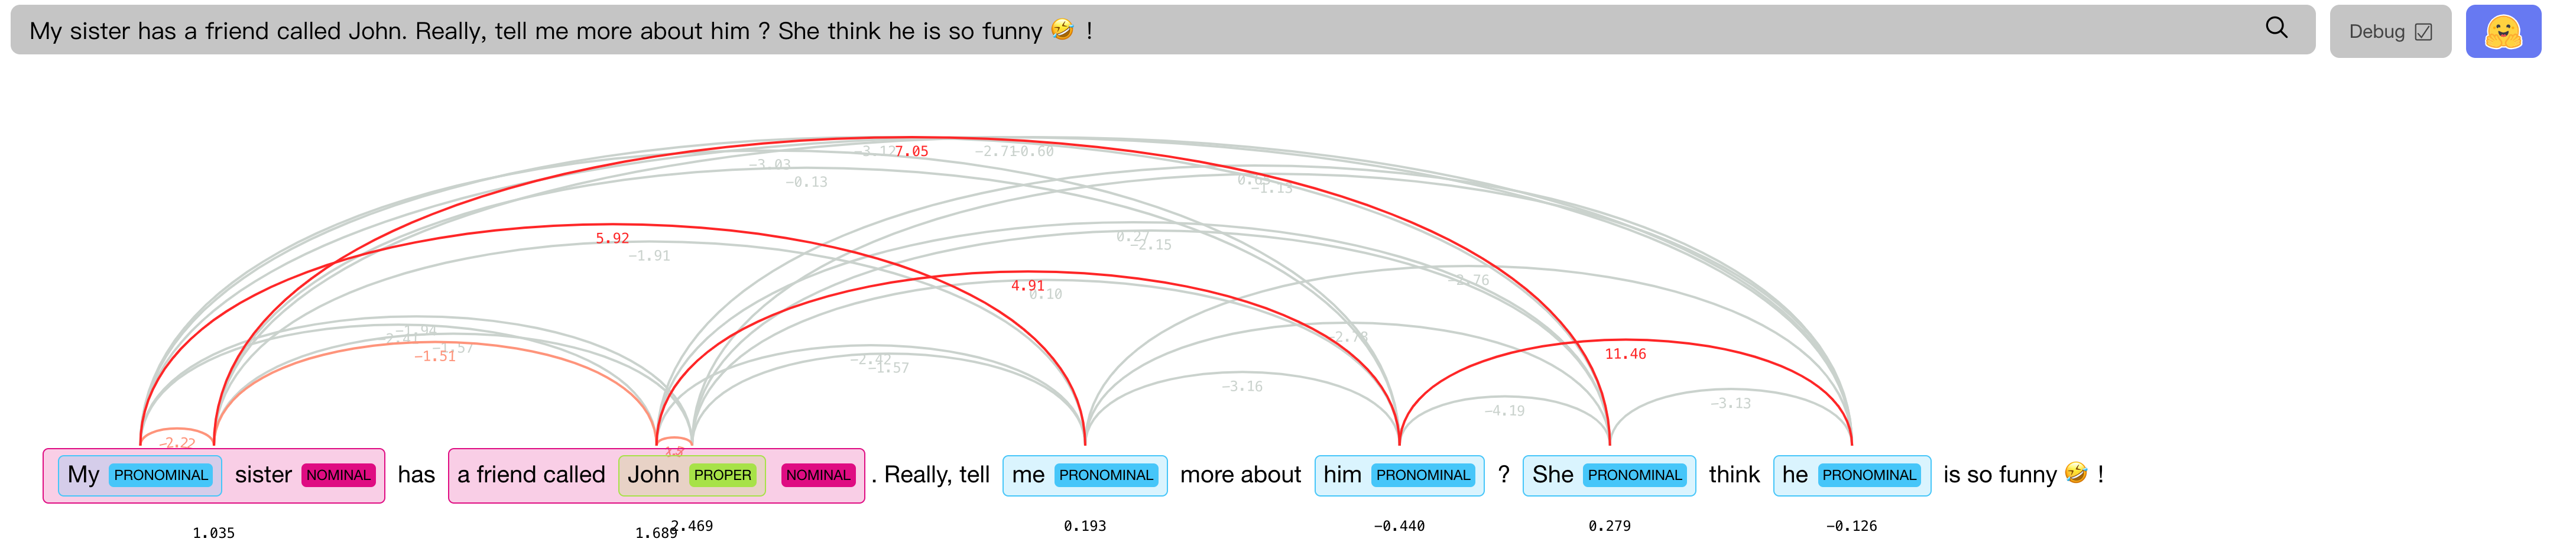
\includegraphics[width=500pt,keepaspectratio]{Coref_visual}
	\caption{Coreference resolution visualized with HuggingFace demo\url{https://huggingface.co/coref/}}
\end{figure}

\subsection{Related Work}

Rule-based In the absence of large-scale data for training coreference models, early systems re- lied heavily on expert knowledge. A frequently used example of this is the Stanford multi-pass sieve system (Lee et al., 2011). A deterministic system, the sieve consists of multiple rule-based models which are applied in succession, from highest-precision to lowest. Gender is among the set of mention attributes identified in the very first stage of the sieve, making this information avail- able throughout the system.

Statistical Statistical methods, often with mil- lions of parameters, ultimately surpassed the performance of rule-based systems on shared task data (Durrett and Klein, 2013; Bjorkelund and Kuhn, 2014). The system of Durrett and Klein (2013) replaced hand-written rules with simple feature templates. Combinations of these features implicitly capture linguistic phenomena useful for resolving antecedents, but they may also unintentionally capture bias in the data. For instance, for occupations which are not frequently found in the data, an occupation+pronoun feature can be highly informative, and the overly confident model can exhibit strong bias when applied to a new domain.

Neural The move to deep neural models led to more powerful antecedent scoring functions, and the subsequent learned feature combinations resulted in new state-of-the-art performance (Wiseman et al., 2015; Clark and Manning, 2016b). Global inference over these models further improved performance (Wiseman et al., 2016; Clark and Manning, 2016a), but from the perspective of potential bias, the information available to the model is largely the same as in the statistical mod- els. A notable exception is in the case of systems which make use of pre-trained word embed- dings (Clark and Manning, 2016b), which have been shown to contain bias and have the potential to introduce bias into the system.

\section{Pronoun Resolution}

Pronoun resolution is part of coreference resolution, the task of identifying for a specified pronoun in a passage, which named entity antecedent it refers to. This is an important task for natural language understanding and a necessary component of machine translation systems, chat bots and assistants.
\begin{figure}[H] % use float package if you want it here
  \centering
  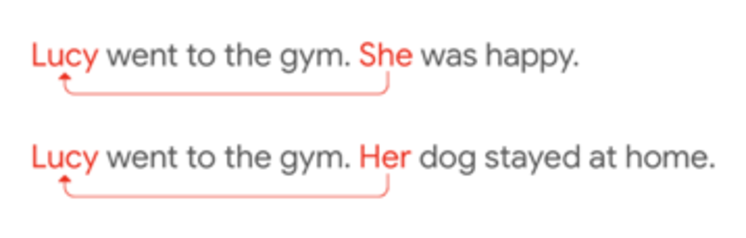
\includegraphics{PR_def.pdf}
  \caption{Pronoun resolution}
  \label{fig:def}
\end{figure}


\section{Gender Bias}

\label{sec:other}

在第~\ref{cha:intro} 章中我们学习了贝叶斯公式~(\ref{equ:chap1:bayes}),这里我们复
习一下:
\begin{equation}
\label{equ:chap2:bayes}
p(y|\vec{x}) = \frac{p(\vec{x},y)}{p(\vec{x})}=
\frac{p(\vec{x}|y)p(y)}{p(\vec{x})}
\end{equation}


\subsection{插图}
\label{sec:graphs}

强烈推荐《\LaTeXe\ 插图指南》!关于子图形的使用细节请参看 \pkg{subcaption} 宏包的说明文档。

\subsubsection{一个图形}
\label{sec:onefig}
一般图形都是处在浮动环境中。之所以称为浮动是指最终排版效果图形的位置不一定与源文
件中的位置对应\footnote{This is not a bug, but a feature of \LaTeX!},这也是刚使
用 \LaTeX{} 同学可能遇到的问题。如果要强制固定浮动图形的位置,请使用 \pkg{float} 宏包,
它提供了 \texttt{[H]} 参数,比如图~\ref{fig:xfig1}。
\begin{figure}[H] % use float package if you want it here
  \centering
  
\includegraphics{thu-whole-logo.pdf}
  \caption{Pronoun Resolution}
  \label{fig:PR}
\end{figure}



\subsubsection{多个图形}
\label{sec:multifig}

如果多个图形相互独立,并不共用一个图形计数器,那么
用 \texttt{minipage} 或者\texttt{parbox} 就可以。否则,请参看
图~\ref{fig:big1-subcaptionbox},它包含两个小图,分别是图~\ref{fig:subfig1}和
图~\ref{fig:subfig2}。推荐使用 \cs{subcaptionbox},因为可以像
图~\ref{fig:big1-subcaptionbox} 那样对齐子图的标题,也可以使用 \pkg{subcaption}
宏包的 \cs{subcaption}(放在 minipage中,用法同\cs{caption})或
是 \pkg{subfigure} 、\pkg{subtable}环境,像图~\ref{fig:big1-subfigure},不要再
用 \cs{subfloat}、\cs{subfigure} 和 \cs{subtable}。

\begin{figure}[h]
  \centering%
  \subcaptionbox{第一个小图形\label{fig:subfig1}}[3cm] %标题的长度,超过则会换行,如下一个小图。
    {
\includegraphics[height=3cm]{thu-fig-logo.pdf}}%
  \hspace{4em}%
  \subcaptionbox{第二个小图形,注意这个图略矮些。如果标题很长的话,它会自动换行\label{fig:subfig2}}
      {
\includegraphics[height=2cm]{thu-text-logo.pdf}}
  \caption{包含子图形的大图形(subcaptionbox示例)}
  \label{fig:big1-subcaptionbox}
\end{figure}
\begin{figure}[h]
  \centering%
  \begin{subfigure}{3cm}
    
\includegraphics[height=3cm]{thu-fig-logo.pdf}
    \caption{第一个小图形}
  \end{subfigure}%
  \hspace{4em}%
  \begin{subfigure}{0.5\textwidth}
    
\includegraphics[height=2cm]{thu-text-logo.pdf}
    \caption{第二个小图形,注意这个图略矮些。subfigure中同一行的子图在顶端对齐。}
  \end{subfigure}
  \caption{包含子图形的大图形(subfigure示例)}
  \label{fig:big1-subfigure}
\end{figure}


如果要把编号的两个图形并排,那么小页就非常有用了:
\begin{figure}
\begin{minipage}{0.48\textwidth}
  \centering
  
\includegraphics[height=2cm]{thu-whole-logo.pdf}
  \caption{并排第一个图}
  \label{fig:parallel1}
\end{minipage}\hfill
\begin{minipage}{0.48\textwidth}
  \centering
  
\includegraphics[height=2cm]{thu-whole-logo.pdf}
  \caption{并排第二个图}
  \label{fig:parallel2}
\end{minipage}
\end{figure}

李氏子蟠,年十七,好古文、六艺,经传皆通习之,不拘於时,学於余。余嘉其能行古
道,作师说以贻之。

\hfill —— 韩愈(唐)
